\documentclass[11pt,a4paper]{article}

\usepackage[T1]{fontenc}
\usepackage[utf8]{inputenc}
\usepackage{graphicx}
\usepackage{booktabs}
\usepackage{amsmath}
\usepackage{geometry}
\usepackage{siunitx}
\usepackage{caption}

\geometry{margin=2.4cm}
\captionsetup{font=small}
\sisetup{detect-all}

\title{RSS-Based Access Point Localization Experiment}
\author{}
\date{}

\begin{document}
\maketitle

\section{Experimental Setup}

This experiment investigates the localization of a single Wi-Fi access point
using received signal strength (RSS) measurements collected inside the Faculty
of Engineering at Ferdowsi University of Mashhad. The target access point was
located in a corridor area of the building. An independently measured coordinate
was kept only as ground truth for final error evaluation:

\begin{center}
\texttt{36 deg 18'46.1"N, 59 deg 31'34.9"E}
\end{center}

which is equivalent to:

\begin{center}
\texttt{latitude = 36.3128055556,\quad longitude = 59.5263611111}.
\end{center}

The building map was drawn from the available JSON map file. In particular, the
room and corridor outlines were reconstructed from the polygon coordinates
stored in the map data.

\section{Data}

The initial dataset used in this experiment is an Excel file containing only the
measurements associated with the selected target access point:

\begin{center}
\texttt{selected\_ap\_b28ba99a8d2a\_pivot\_data.xlsx}
\end{center}

This file is stored in the output directory of the experiment and contains two
sheets:

\begin{itemize}
\item \texttt{selected\_ap\_samples}: the measurement records used for
localization;
\item \texttt{summary}: a compact summary of the selected access point and its
RSS statistics.
\end{itemize}

The sample sheet contains the measurement coordinates, device and orientation
metadata, and one RSS column for the selected access point. RSS measurements
from other access points are not included. The RSS column is named:

\begin{center}
\texttt{selected\_ap\_rss\_dbm}
\end{center}

The selected access point is:

\begin{center}
\texttt{BSSID = b28ba99a8d2a}
\end{center}

\begin{table}[h]
\centering
\caption{Summary of the Excel dataset used in the experiment.}
\label{tab:data-summary}
\begin{tabular}{lr}
\toprule
Quantity & Value \\
\midrule
Access point BSSID & \texttt{b28ba99a8d2a} \\
Number of valid RSS samples & 1069 \\
Maximum RSS & \SI{-29.0}{dBm} \\
Mean RSS & \SI{-72.89}{dBm} \\
Minimum RSS & \SI{-98.0}{dBm} \\
\bottomrule
\end{tabular}
\end{table}

The valid measurements cover the corridor region around the selected access
point and nearby spaces. Figure~\ref{fig:rss-map} shows the RSS samples overlaid
on the building map. Stronger RSS values are shown using green shades, while
weaker RSS values are shown using red shades.

\begin{figure}[h]
\centering
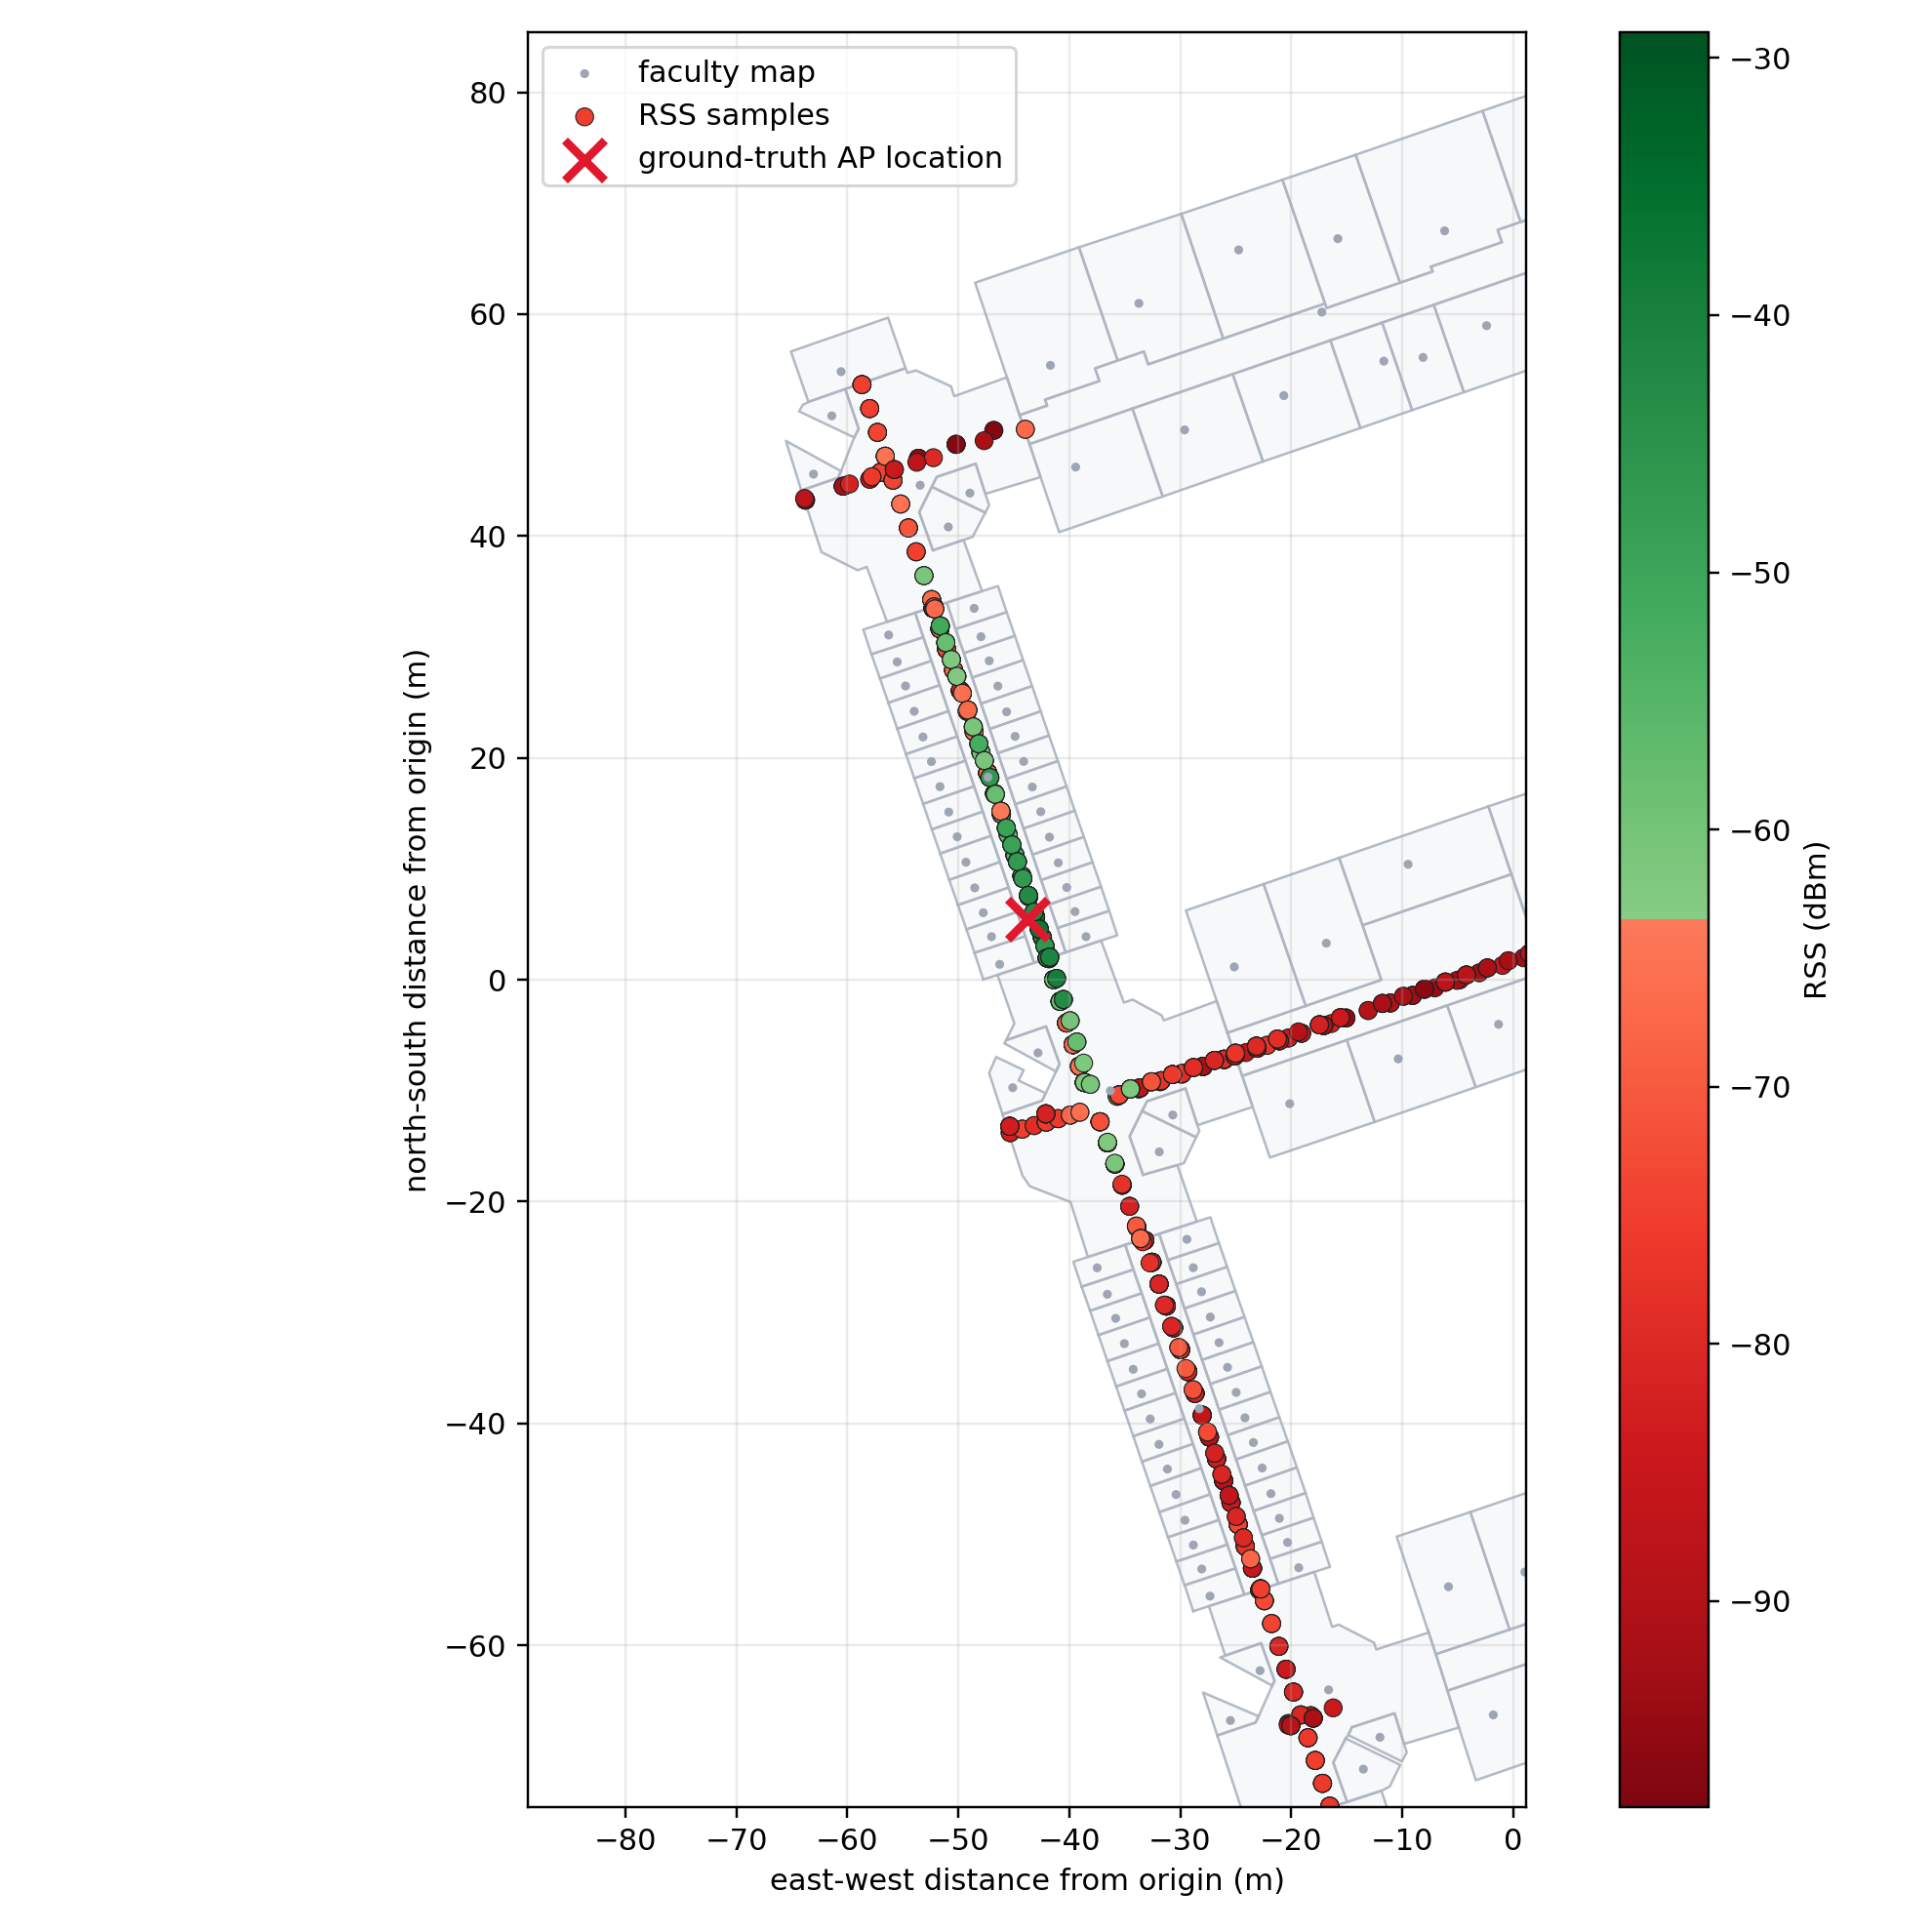
\includegraphics[width=0.92\textwidth]{figures/rss_map.png}
\caption{RSS measurements of the selected access point overlaid on the building map.}
\label{fig:rss-map}
\end{figure}

\section{Initialization and Ground-Truth Evaluation}

The ground-truth coordinate was not used to initialize or constrain the fitting
procedure. As a simple RSS-only initialization, the measurement point with the
maximum RSS was used as the initial AP position. For descriptive analysis, the
RSS samples were also summarized by an RSS-weighted centroid. For a sample with
RSS value \(r_i\), the weight was defined as:

\begin{equation}
w_i = 10^{(r_i-r_{\max})/10},
\end{equation}

where \(r_{\max}\) is the strongest RSS value in the dataset. The corresponding
weighted centroid was computed as:

\begin{equation}
x_c = \frac{\sum_i w_i x_i}{\sum_i w_i},
\qquad
y_c = \frac{\sum_i w_i y_i}{\sum_i w_i}.
\end{equation}

For this dataset, the RSS-weighted centroid was approximately
\SI{1.37}{m} away from the ground-truth coordinate. This indicates that
the strongest RSS measurements are spatially concentrated around the expected
access point location.

\section{RSS Fitting Model}

The access point location was estimated by fitting a log-distance path-loss
model to the RSS measurements. The model is:

\begin{equation}
RSS(d) = RSS_{1m} - 10n\log_{10}(d),
\end{equation}

where \(RSS_{1m}\) denotes the RSS at one meter, \(n\) is the path-loss exponent,
and \(d\) is the Euclidean distance between a measurement point and the estimated
access point position.

The unknown parameter vector was:

\begin{equation}
\theta = (x_{AP}, y_{AP}, RSS_{1m}, n).
\end{equation}

For a measurement point \(i\) with local Cartesian coordinate \((x_i,y_i)\),
the distance to a candidate AP location is:

\begin{equation}
d_i(\theta)=\max\left(\sqrt{(x_i-x_{AP})^2+(y_i-y_{AP})^2}, 1\right).
\end{equation}

The lower bound of \SI{1}{m} avoids numerical instability in the logarithm
when a candidate AP location becomes very close to a measurement point. The
model-predicted RSS at point \(i\) is then:

\begin{equation}
\widehat{r}_i(\theta)=RSS_{1m}-10n\log_{10}\left(d_i(\theta)\right),
\end{equation}

and the residual is defined as:

\begin{equation}
e_i(\theta)=\widehat{r}_i(\theta)-r_i,
\end{equation}

where \(r_i\) is the measured RSS value. Instead of minimizing the ordinary
sum of squared residuals directly, a robust nonlinear least-squares objective
was used:

\begin{equation}
\min_{\theta}\; \frac{1}{2}\sum_{i=1}^{N}\rho\left(e_i(\theta)^2\right).
\end{equation}

The robust loss was the \texttt{soft\_l1} loss, defined as:

\begin{equation}
\rho(z)=2\left(\sqrt{1+z}-1\right).
\end{equation}

For small residuals, this loss behaves similarly to the squared loss. For large
residuals, its growth is slower, so unusually noisy RSS samples have less
influence on the final AP estimate. This is useful for indoor RSS measurements,
where multipath propagation, shadowing, and device orientation can produce
occasional outliers.

The fitting procedure was performed as follows:

\begin{enumerate}
\item First, all measurement coordinates were converted from latitude and
longitude to a local Cartesian coordinate system in meters. This made it possible
to compute Euclidean distances between the candidate AP location and each RSS
measurement point.

\item Next, only valid RSS observations of the selected AP were used. In this
dataset, valid observations are the 1069 samples listed in the Excel file.

\item The initial AP location for the optimizer was set to the measurement point
with the maximum RSS value. This choice uses only the RSS dataset and does not
use the ground-truth coordinate.

\item The initial value of \(RSS_{1m}\) was set from a high RSS percentile of the
data, and the initial path-loss exponent was set to \(n=2\).

\item Bound constraints were used to keep the solution physically meaningful.
The AP coordinates were allowed to move within the measurement region with an
additional margin, \(RSS_{1m}\) was constrained to a realistic RSS interval, and
the path-loss exponent was constrained to \(0.5 \le n \le 6\).

\item For each candidate parameter vector
\(\theta=(x_{AP},y_{AP},RSS_{1m},n)\), the distance from the candidate AP
location to every measurement point was computed. The log-distance model then
predicted the RSS value at each point.

\item At each iteration, the optimizer evaluated the residual vector
\(\mathbf{e}(\theta)\), applied the robust loss, and updated the four unknowns
\((x_{AP},y_{AP},RSS_{1m},n)\) to reduce the objective function. The process
continued until the change in the objective became sufficiently small.

\item Finally, the optimized AP coordinate was converted back from the local
Cartesian coordinate system to latitude and longitude. The ground-truth
coordinate was used only at this final stage to compute the localization error.
\end{enumerate}

\section{Localization Results}

Table~\ref{tab:fit-result} reports the fitted model parameters and the estimated
access point location.

\begin{table}[h]
\centering
\caption{Estimated AP location and fitted RSS model parameters.}
\label{tab:fit-result}
\begin{tabular}{lr}
\toprule
Quantity & Value \\
\midrule
Initial latitude & 36.3127978000 \\
Initial longitude & 59.5263734000 \\
Estimated latitude & 36.3128106176 \\
Estimated longitude & 59.5263414105 \\
Distance from ground truth & \SI{1.85}{m} \\
Estimated \(RSS_{1m}\) & \SI{-28.36}{dBm} \\
Path-loss exponent \(n\) & 3.22 \\
RSS RMSE & \SI{8.53}{dB} \\
RSS MAE & \SI{6.91}{dB} \\
\bottomrule
\end{tabular}
\end{table}

Figure~\ref{fig:estimated-map} shows the ground-truth coordinate and the estimated
location on the building map. The red cross marks the ground-truth coordinate, and
the black star marks the estimated access point position.

\begin{figure}[h]
\centering
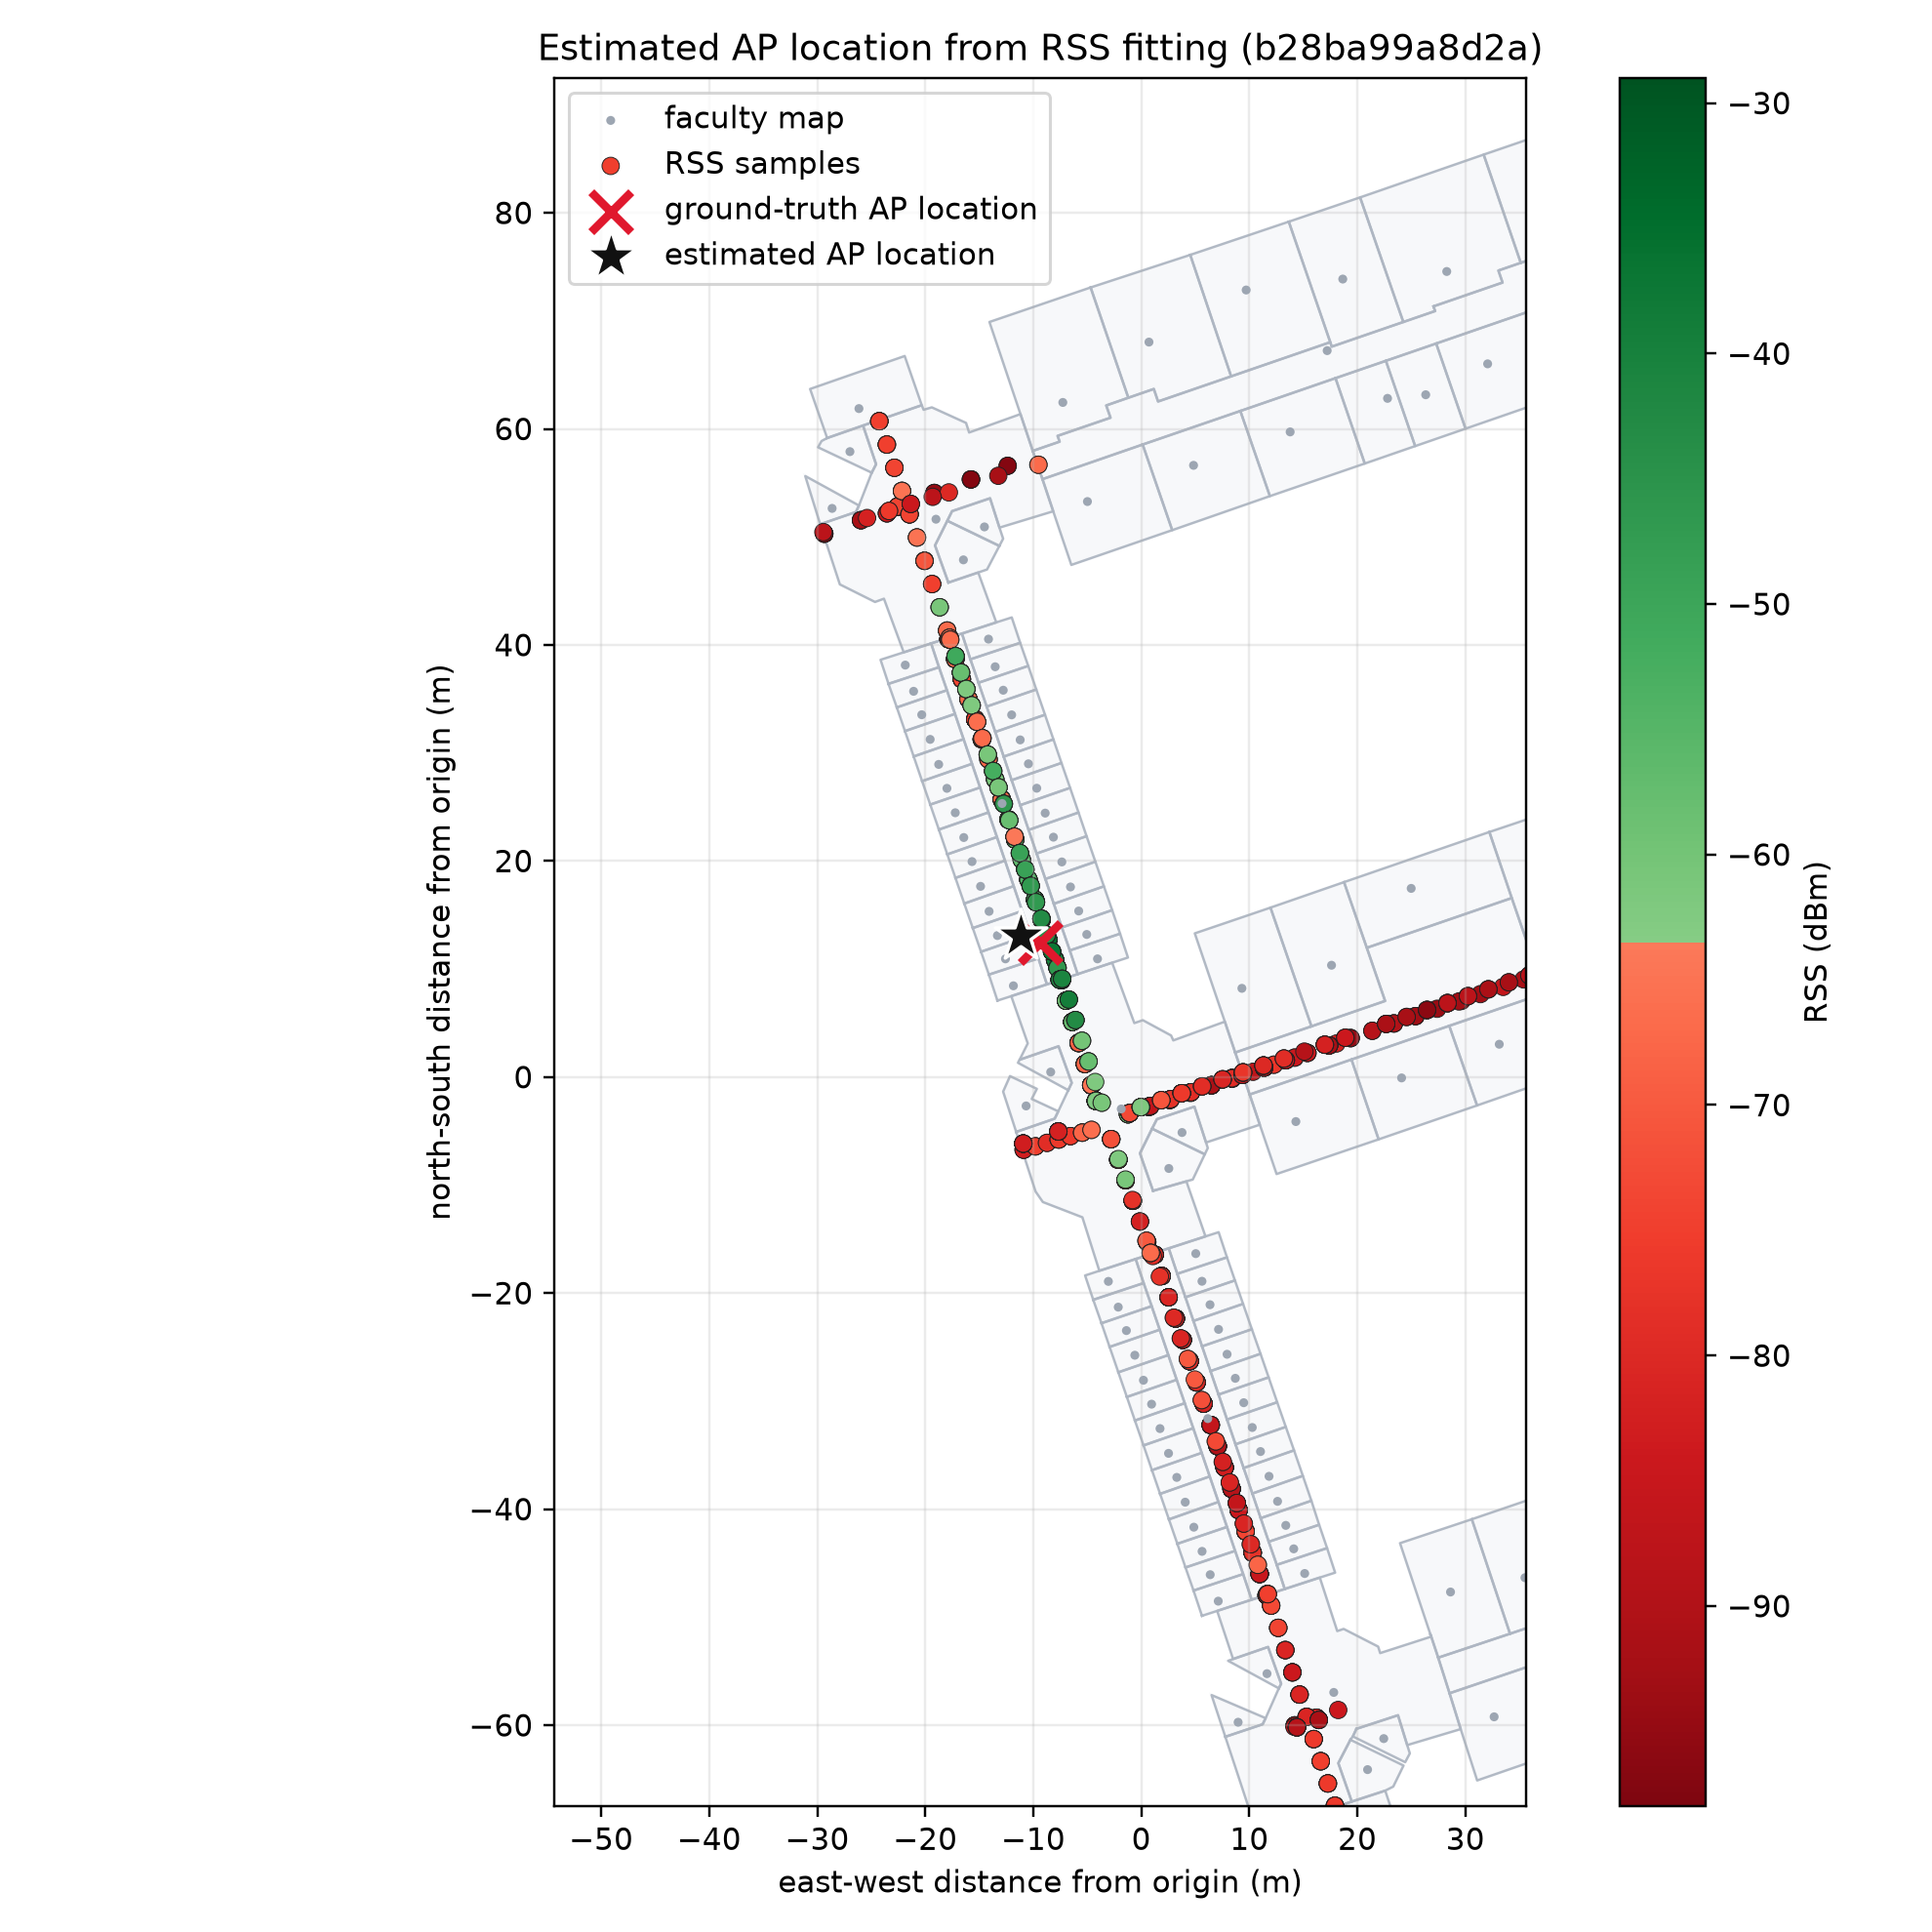
\includegraphics[width=0.92\textwidth]{figures/estimated_ap_map.png}
\caption{Reference and estimated access point locations on the building map.}
\label{fig:estimated-map}
\end{figure}

The estimated location was approximately \SI{1.85}{m} away from the ground-truth
coordinate. Given the variability of indoor RSS measurements, this result shows
that the log-distance fitting model provides a practical approximation of the
access point position when a sufficient number of measurements are available in
the surrounding corridor area.

\end{document}
